% use paper, or submit
% use 11 pt (preferred), 12 pt, or 10 pt only

\documentclass[letterpaper, preprint, paper,11pt]{AAS}	% for preprint proceedings
%\documentclass[letterpaper, paper,11pt]{AAS}		% for final proceedings (20-page limit)
%\documentclass[letterpaper, paper,12pt]{AAS}		% for final proceedings (20-page limit)
%\documentclass[letterpaper, paper,10pt]{AAS}		% for final proceedings (20-page limit)
%\documentclass[letterpaper, submit]{AAS}			% to submit to JAS

\usepackage{bm}
\usepackage{amsmath}
\usepackage{subfigure}
%\usepackage[notref,notcite]{showkeys}  % use this to temporarily show labels
\usepackage[colorlinks=true, pdfstartview=FitV, linkcolor=black, citecolor= black, urlcolor= black]{hyperref}
\usepackage{overcite}
\usepackage{footnpag}			      	% make footnote symbols restart on each page

% Added packages 2019 Feb 17
\usepackage{float}
\usepackage{amssymb}
%\usepackage{graphicx} % Allows including images
%\usepackage{mathrsfs}
%\usepackage{booktabs} % Allows the use of \toprule, \midrule and \bottomrule in tables



\PaperNumber{XX-XXX}



\begin{document}
	
	\title{SUN-AVOIDANCE SLEW PLANNING ALGORITHM WITH POINTING AND ACTUATOR CONSTRAINTS}
	
	\author{
		Mohammad Ayoubi\thanks{Title, department, affiliation, postal address.} and Junette Hsin\thanks{Title, department, affiliation, postal address.}
	}
	
	
	\maketitle{} 		
	
	
	\begin{abstract}
		
		A sun avoidance slew maneuver is described in this paper. The algorithm finds the angular velocity, angular acceleration, and quaternion profiles needed to avoid the sun vector that lies near the plane of a sensor's FOV onboard a spacecraft. 
		
		% The abstract should briefly state the purpose of the manuscript, the problem to be addressed, the approach taken, and the nature of results or conclusions that can be expected. It should stand independently and tell enough about the manuscript to permit the reader to decide whether the subject is of specific interest. The abstract shall be typed single space, justified, centered, and with a column width of 4.5 inches. The abstract is not preceded by a heading of ``Abstract'' and its length may not extend beyond the first page.
		
	\end{abstract}
	
	\section{Introduction}
	Large-angle slew maneuvers are required during any Earth-pointing or interplanetary missions. In many space missions, and for safety consideration, a sensitive payload such as imaging camera or telescope needs to be retargeted while avoiding sun vector or other bright objects in the sky.
	The attitude reorientation problem in the presence of attitude constrained zones has been studied in the last three decades. McInnes\cite{McInnes1994} addressed this problem via using an artificial potential function. He proposed a guidance law which is entirely analytical and suitable for onboard implementation. However, he uses Euler angles which are singular for large slew angles. 
	A geometric approach was proposed by Spindle\cite{Spindler1998}, Hablani\cite{Hablani1998}, and Biggs and Colley\cite{Biggs2016}  where a feasible attitude maneuver, or a guidance law, is precomputed based on the attitude-avoidance-zone constraints.  Another approach for addressing this problem is using randomized algorithms\cite{Frazzoli01}. However, depends on the number of constraints and initial and final attitudes, this approach is computationally expensive and not suitable for onboard implementation. Another approach for solving the time optimal reorientation maneuver subject to boundaries and path constraints is proposed by Spiller et al.\cite{Spiller2016}. They used the particle swarm optimization (PSO) technique to find a sub-optimal solution with keep-out constraints. Another approach is to cast the problem as a convex optimization problem and use a semi-definite programming (SDP) or  quadratically constrained quadratic programming (QCQP) to solve them.  See for instance Kim and Mesbahi\cite{Kim2004}, Kim et al.\cite{Kim2010}, Sun and Dai\cite{Sun2015}, and Lee and Mesbahi\cite{Lee2014} %proposed a new method for time and energy optimal path planning in the presence of attitude constrained zones using unit quaternions. They solved their open-loop optimal control problem using Guass pseudospectral method. 
	Recently, Ramos and Schaub\cite{Ramos2018} proposed a method based on the Lyapunov stability theorem and logarithmic barrier potential function to derive a steering law for attitude control of a spacecraft subject to conically constrained inclusion and exclusion regions. They also considered the control-torque constraint in their algorithm.  
	In this paper, we present a novel geometric approach for large-angle slew planning with pointing and actuator constraints.  We assume spacecraft has a single light-sensitive payload with control-torque and angular momentum constraints. Furthermore, we assume the initial and final attitudes, instrument boresight vector, and sun vector are known. Then we derive the desired quaternions, angular velocity, and angular acceleration based on the Pontryagin's minimum principle (PMP) for this maneuver. The proposed algorithm in this paper is intuitive, deterministic, easy to implement, and includes the control-torque and angular momentum constraints. The main drawback of the proposed algorithm is its limitation for a single payload, single-constraint region.  A Monte Carlo simulation is performed to show the viability of the proposed algorithm with control-torque and angular momentum constraints. 
	
	%-------------------------------------------------------------------------------------------------------------------------------------------------------------------
	
	\subsection{Problem Justification}
	
	Given:$_N\hat{P}_i$, $_N\hat{P}_f$, $_N\hat{S}$, $_G\hat{P}$, $\epsilon_p$, $^Nq^G$, $^N_G\omega^G(t_i)$, and $^N_G\omega^G(t_f)$ .\\
	%Assumption: The spacecraft is rigid.\\
	
	Find: 
	\begin{enumerate}
		\item A sequence of slew maneuvers to avoid sun vector.
		\item the commanded angular velocity, angular acceleration, and quaternion profiles.
	\end{enumerate} 
	\begin{figure}[htb]
		\begin{center}
			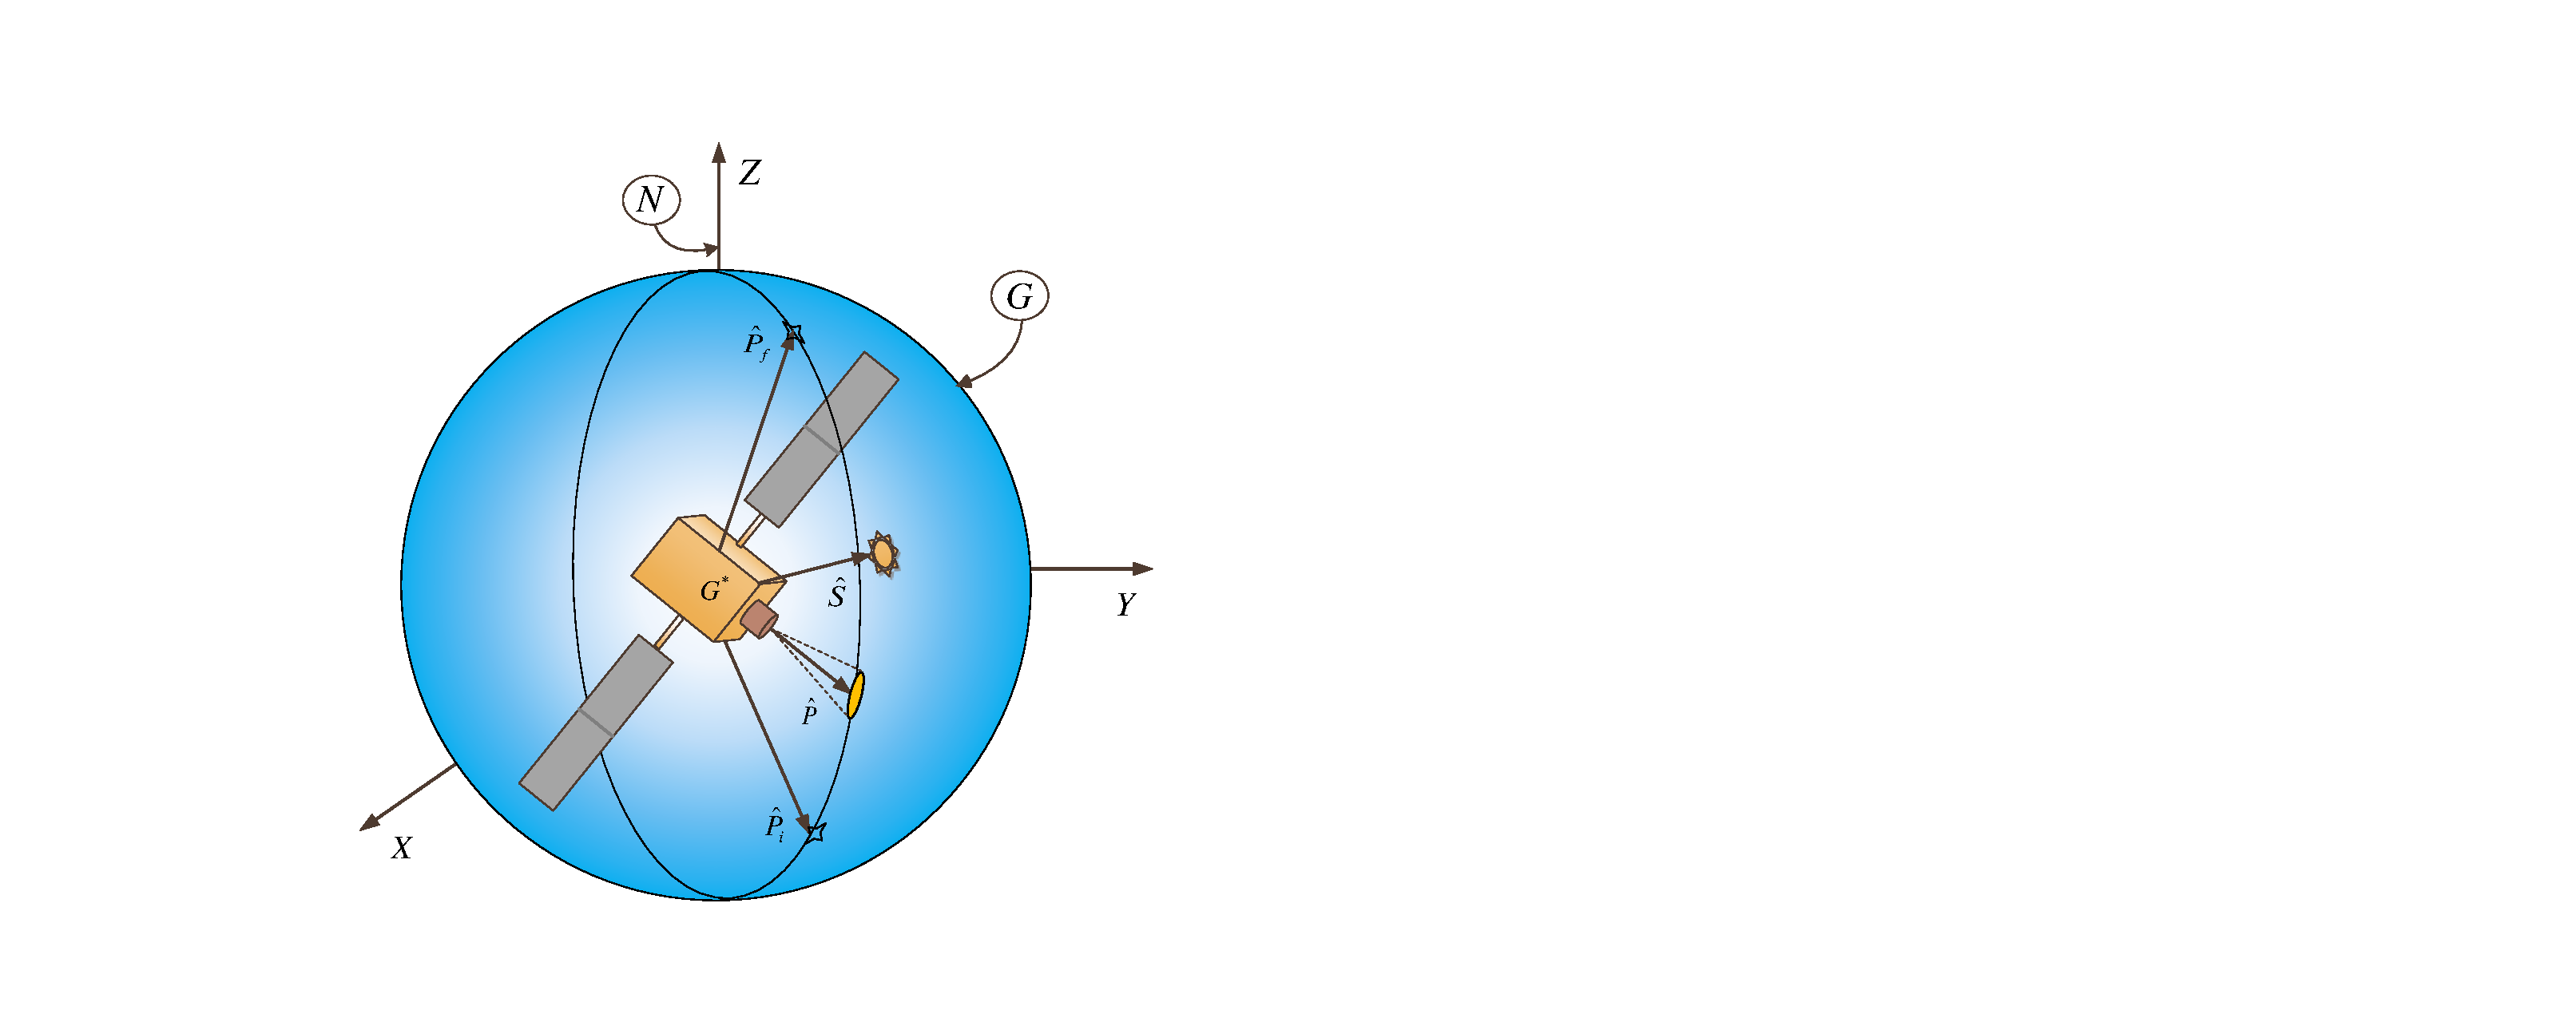
\includegraphics[width=6in]{./Figures/SAS_Schematic}
			\caption{The spacecraft is not drawn to scale.}
		\end{center}
	\end{figure}
	
	%-------------------------------------------------------------------------------------------------------------------------------------------------------------------
	
	Nomenclature: 
	\begin{itemize}
		\item $G$ frame: Unit sphere attached to the gyrostat.
		\item $N$: frame: The Newtonian frame fixed in the inertial space.
		\item $_G\hat{P}$: Unit vector along the bore sight of payload in the $G$ frame.
		\item $_N\hat{P}_i$: Unit vector of the initial point in the $G$ frame.
		\item $_N\hat{P}_f$: Unit vector of the final point in the $G$ frame.
		\item $_N\hat{S}$: Unit vector of the sun vector in the $N$ frame.
		\item $\epsilon_p$: Payload half-cone angle.
	\end{itemize}
	
	%-------------------------------------------------------------------------------------------------------------------------------------------------------------------
	
	\clearpage
	\subsection{Literature surveyed}
	
	This is the literature surveyed. 
	
	\subsection{Contribution of work} 
	
	This is the contribution of work. 
	
	\section{Algorithm Description} 
	
	\subsection{Slew Maneuver} 
	
	%-------------------------------------------------------------------------------------------------------------------------------------------------------------------
	
	\subsubsection{Check the Sun Vector Intrusion}
	\begin{enumerate}
		\item Check the angular separation between the sun vector, $\hat{S}$, and the $\hat{P}_i-\hat{P}_f$ plane.
		\begin{equation}
		\alpha=\frac{\pi}{2}-\cos^{-1}(\hat{S}.\hat{e})
		\end{equation}
		where the eigenaxis is determined by
		\begin{equation}\label{eaxis}
		\hat{e}=\frac{\hat{P}_i\times\hat{P}_f}{|\hat{P}_i\times \hat{P}_f|}
		\end{equation} 
		
		\item IF $|\alpha|<\epsilon_p$,THEN determine the projection of the sun vector into the $\hat{P}_i-\hat{P}_f$ plane.
		\begin{equation}\label{Sbar}
		\vec{S}_{||}=\hat{S}\cos\alpha
		\end{equation}
	\end{enumerate}
	
	%-------------------------------------------------------------------------------------------------------------------------------------------------------------------
	
	\subsubsection{Slew Maneuvers}
	
	\begin{enumerate}
		\item The $1^{st}$ slew around the eigenaxis,$\hat{e}$, through angle:
		%		\end{enumerate}
		\begin{equation}
		\phi_1=\left\{
		\begin{array}{ll}
		\cos^{-1}(\hat{P}._G\hat{S}_{||})-\epsilon_p& when\  \cos^{-1}(\hat{P}._G\hat{S}_{||})-\epsilon_p\leq \pi\\
		\cos^{-1}(\hat{P}._G\hat{S}_{||})-\epsilon_p-2\pi& when\ \cos^{-1}(\hat{P}._G\hat{S}_{||})-\epsilon_p>\pi\\
		\end{array}
		\right.
		\end{equation}
		\begin{figure}[htb]
			\begin{center}
				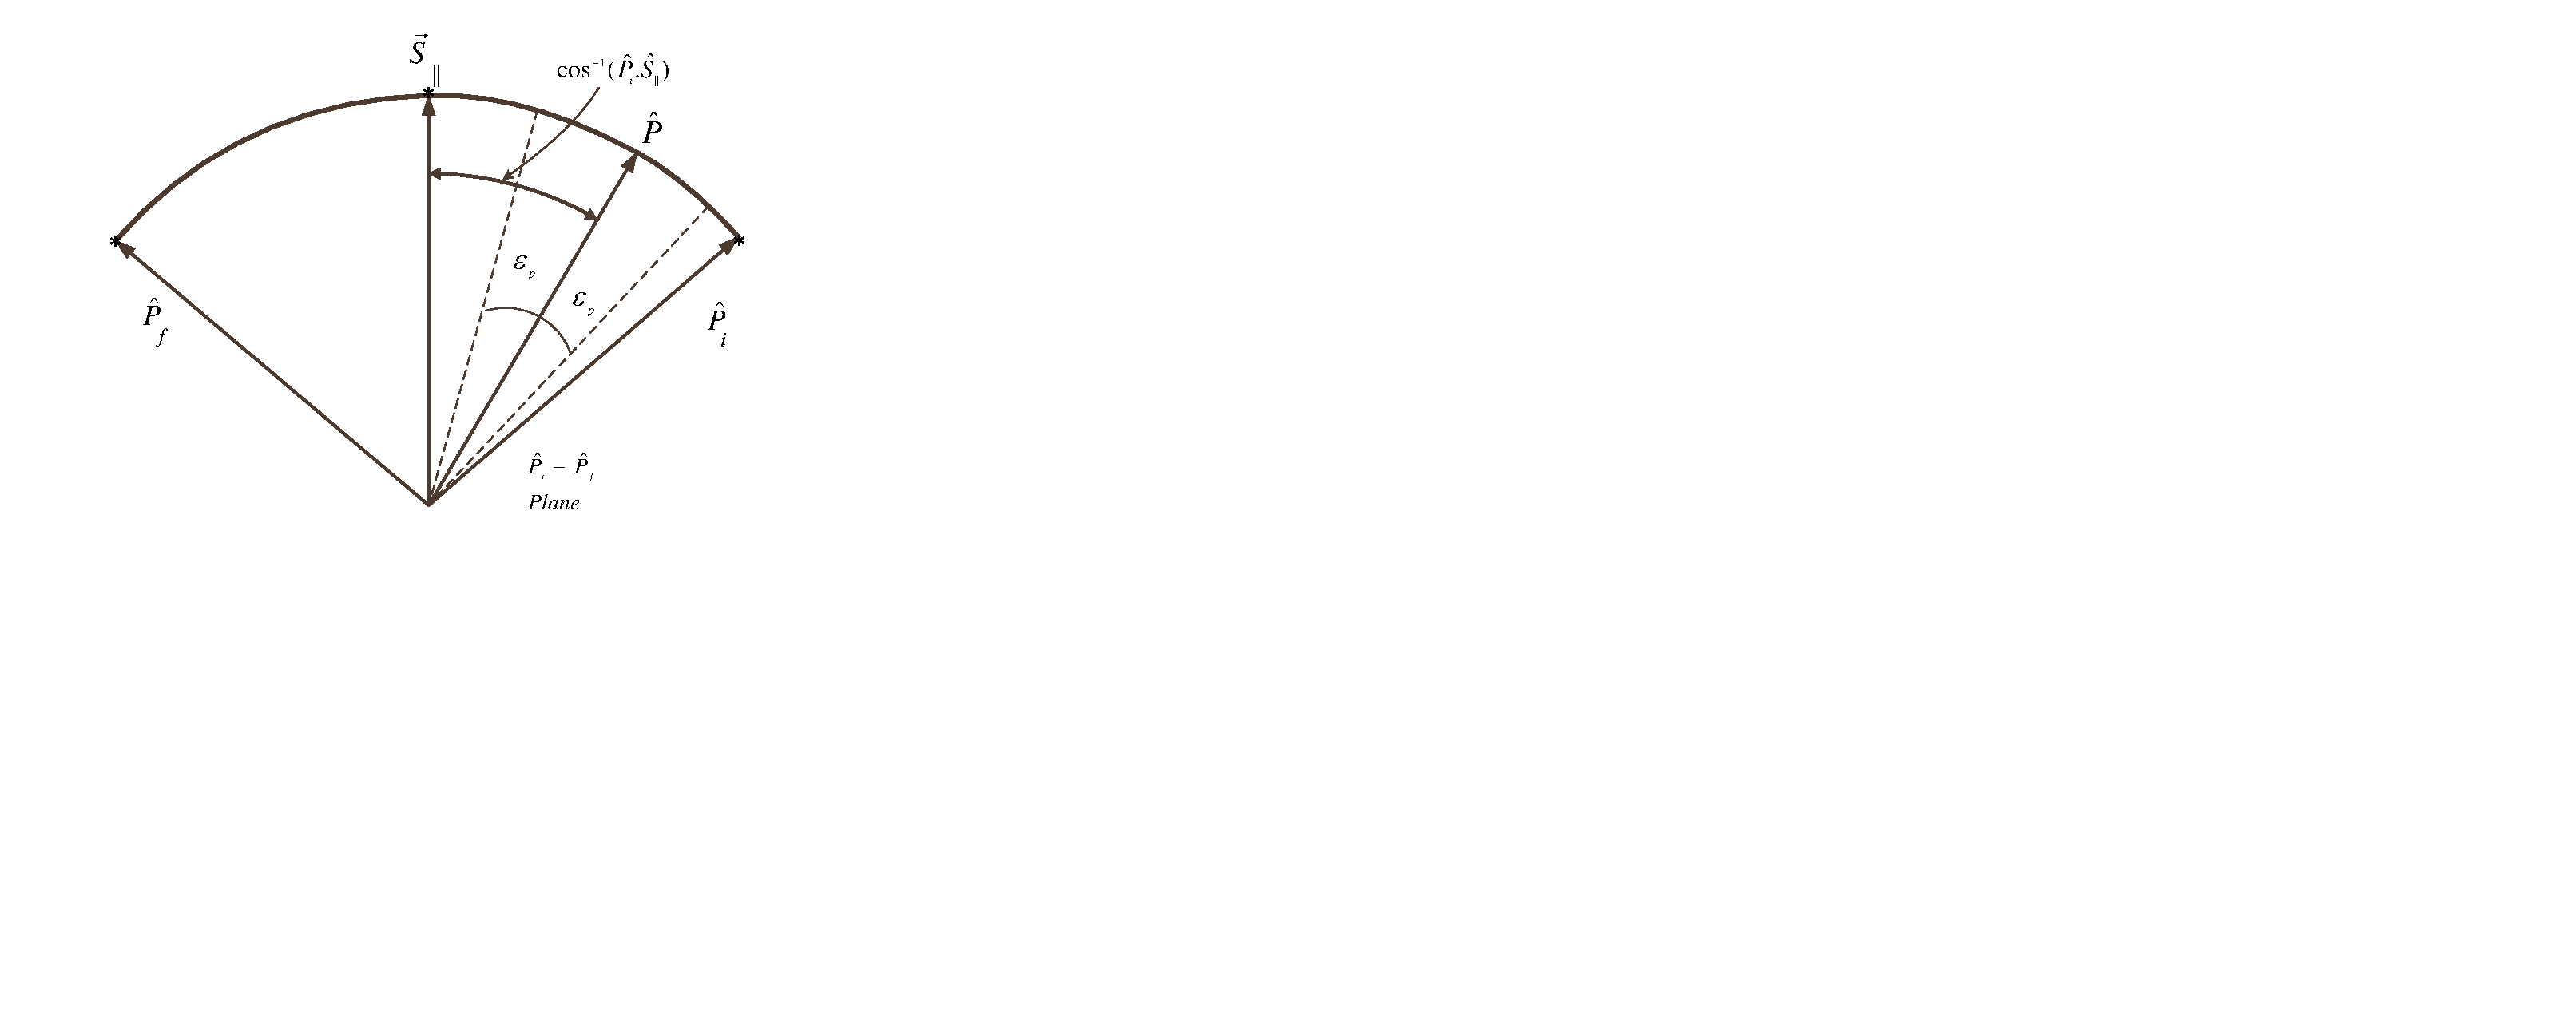
\includegraphics[width=2.3in]{./Figures/SVAS_1r}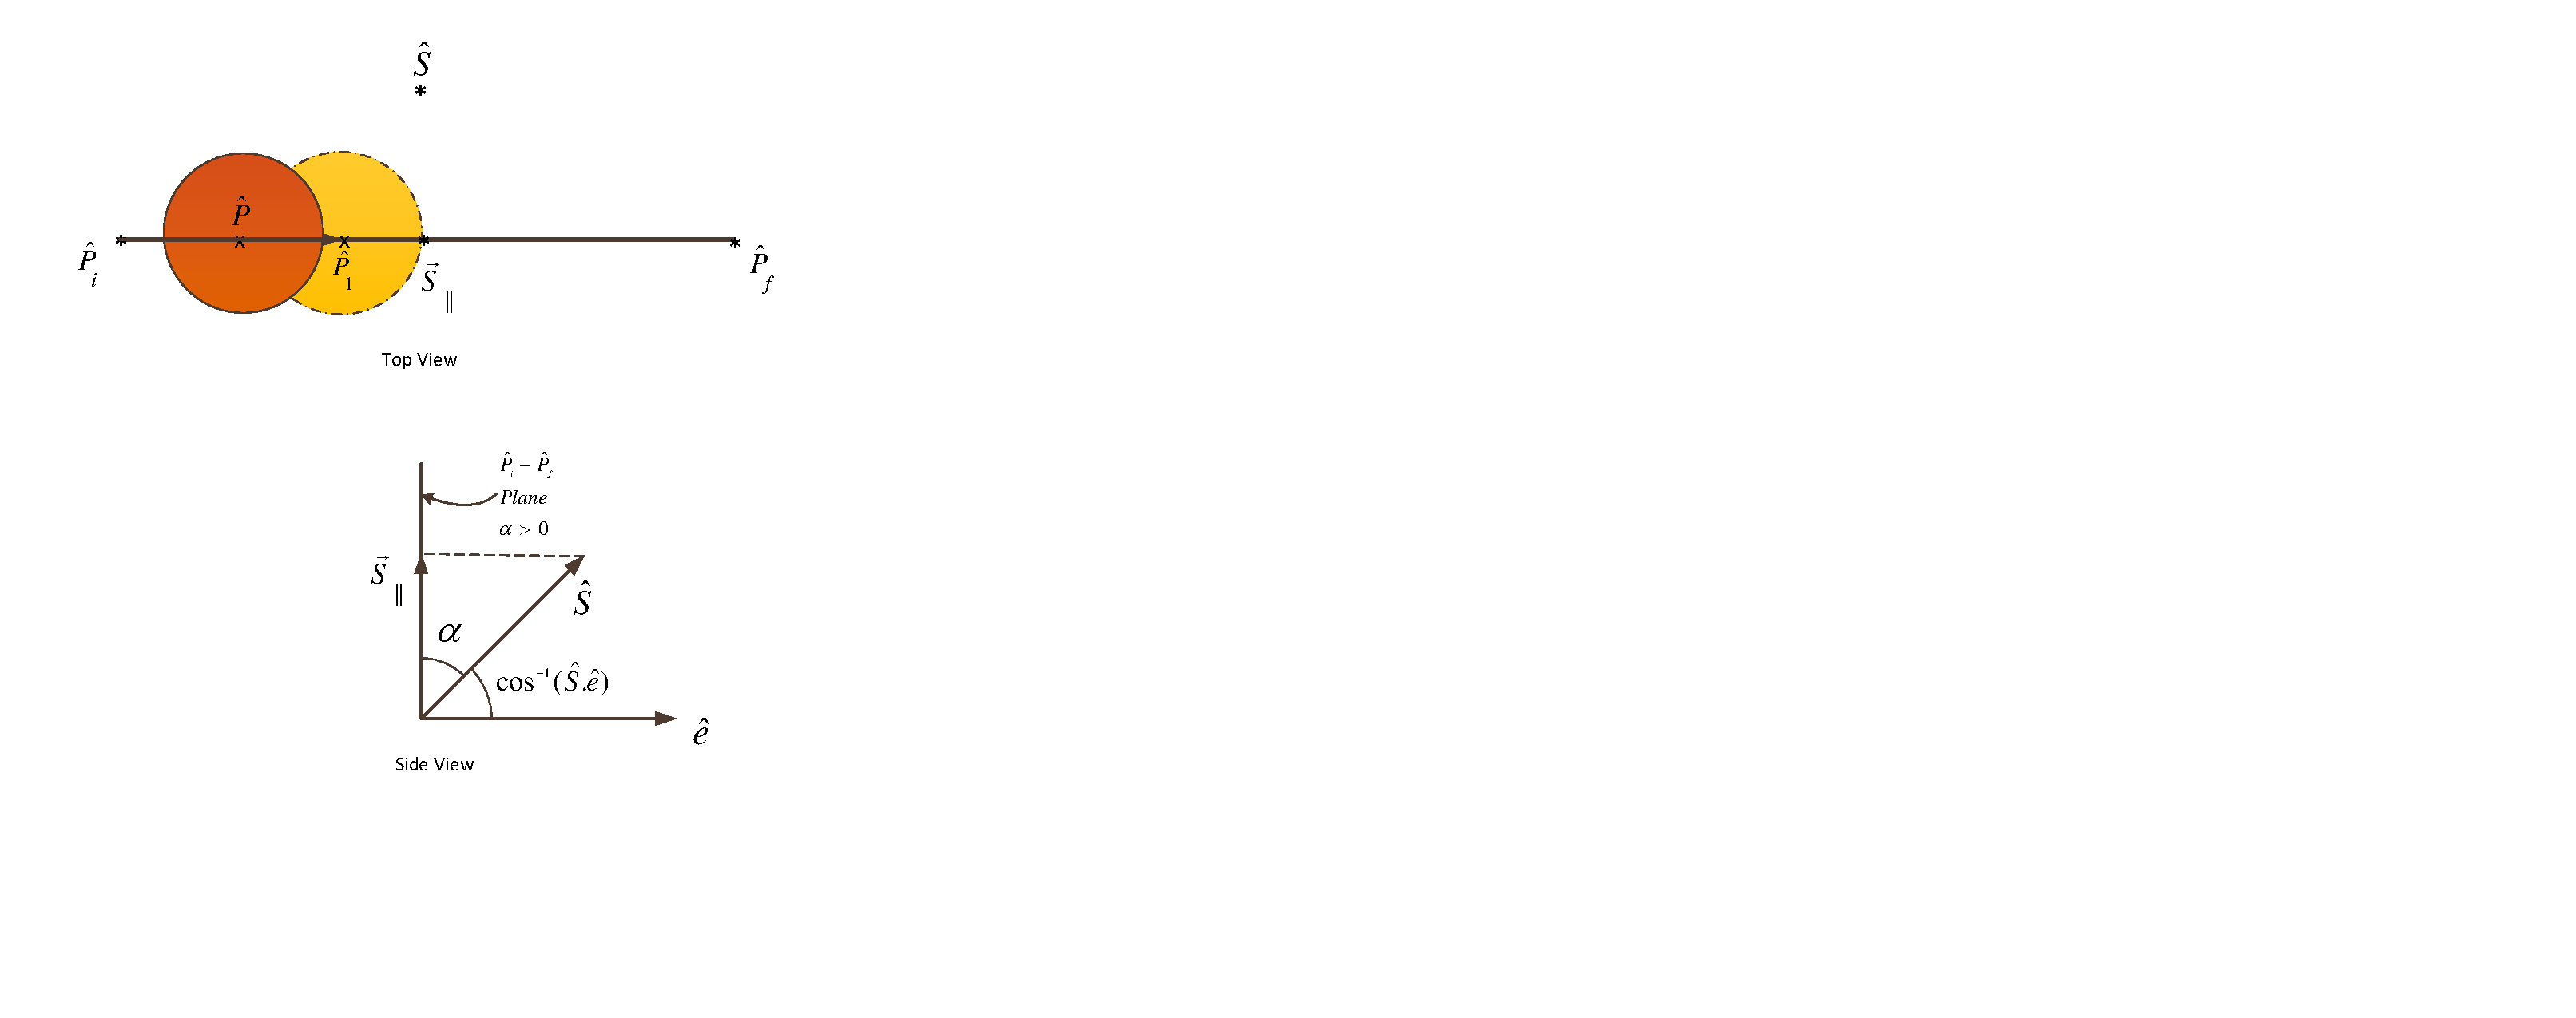
\includegraphics[width=2.3in]{./Figures/SVAS_1rb}
			\end{center}
		\end{figure}
		
		%-------------------------------------------------------------------------------------------------------------------------------------------------------------------
		
		%	\begin{enumerate}[2]
		\item The $2^{nd}$ slew around the unit sun vector, $\hat{S}$, via $\phi_2$.
		\begin{enumerate}
			\item when $\alpha\neq0$
			%		\end{enumerate}
			%	\end{enumerate}
			\begin{figure}[H]
				\begin{center}
					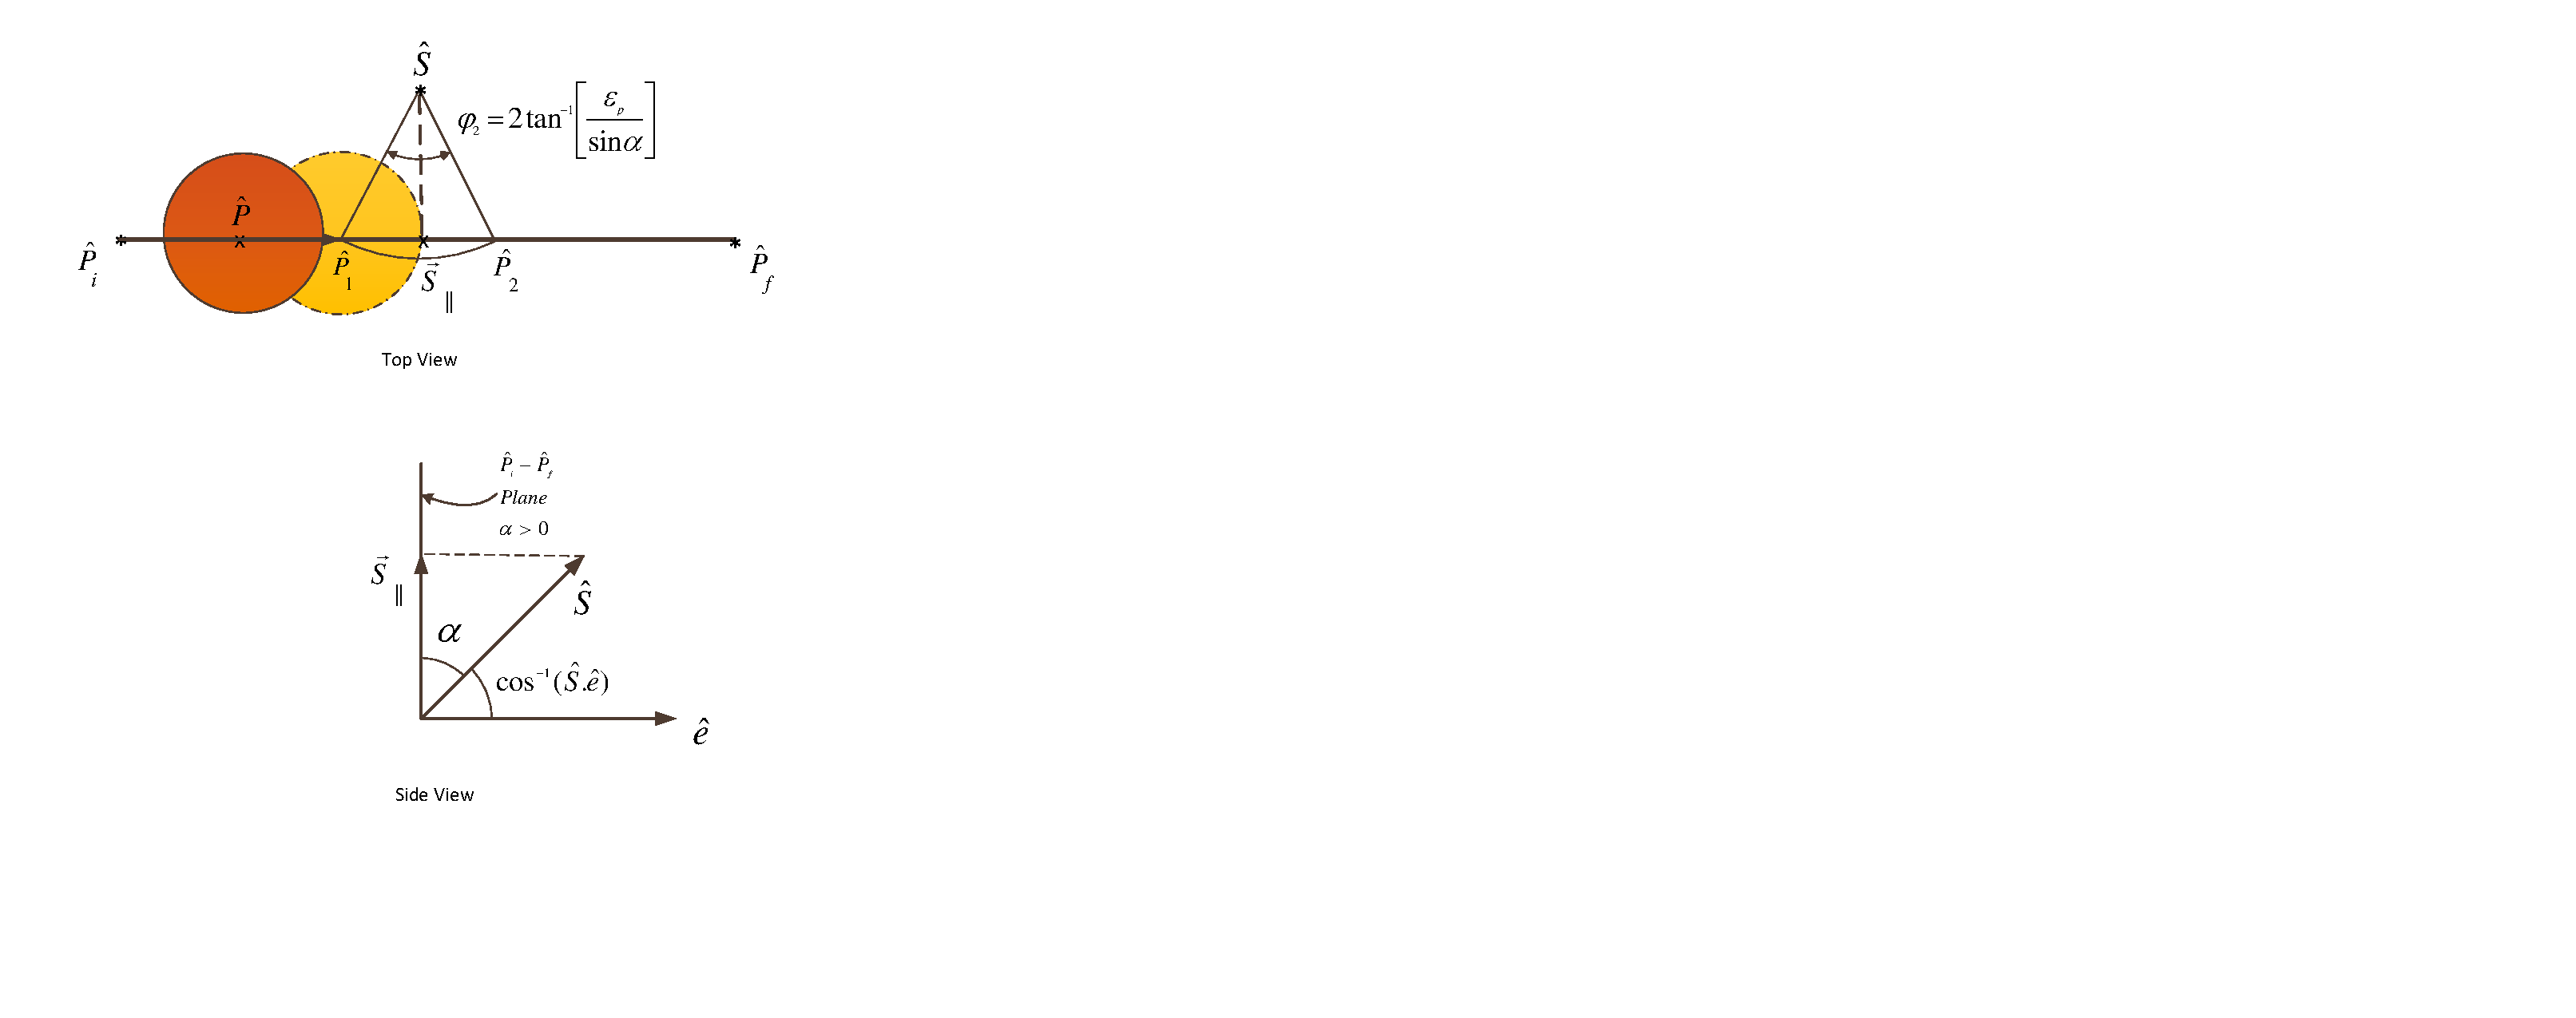
\includegraphics[width=2.3in]{./Figures/SVAS_2r}
				\end{center}
			\end{figure}
			
			%-------------------------------------------------------------------------------------------------------------------------------------------------------------------
			
			%	\begin{enumerate}[2]
			%		\item The $2^{nd}$ slew around the unit sun vector, $\hat{S}$, via $\phi_2=180^{\circ}$.
			%		\begin{enumerate}[b)]
			\item when $\alpha=0$
			%		\end{enumerate}
			%	\end{enumerate}
			\begin{figure}[H]
				\begin{center}
					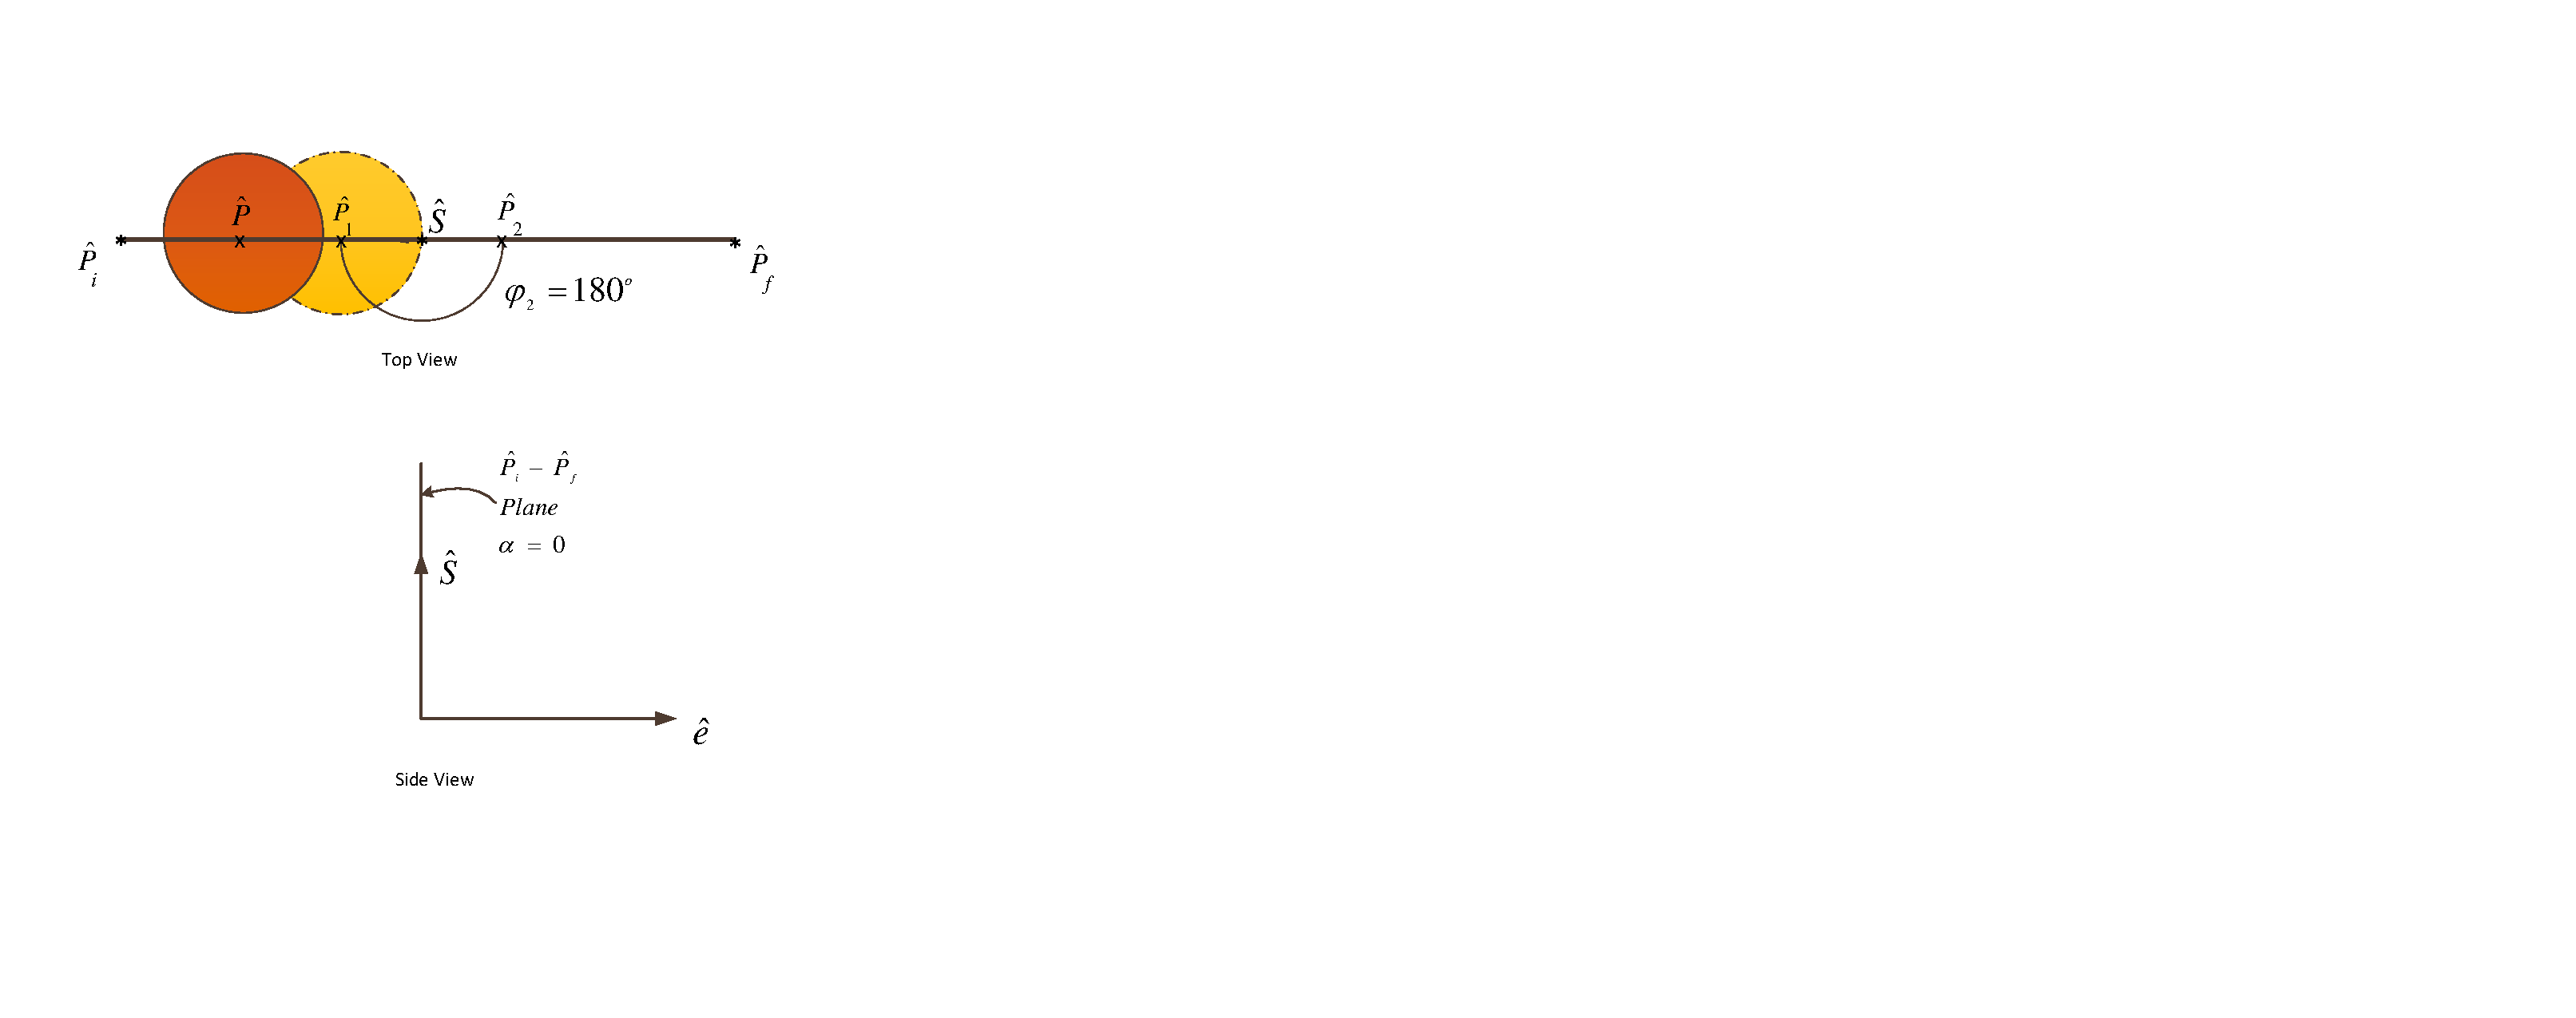
\includegraphics[width=2.3in]{./Figures/SVAS_3r}
				\end{center}
			\end{figure}
		\end{enumerate}
		
		%-------------------------------------------------------------------------------------------------------------------------------------------------------------------
		
		\item The $3^{rd}$ slew about the $\hat{e}$ through angle:
		\begin{equation}
		\phi_3=\left\{
		\begin{array}{ll}
		\cos^{-1}(_G\hat{P}_f.\hat{P}_2)& when\  _G\hat{P}_f.\hat{P}_2\geq 0\\
		\cos^{-1}(_G\hat{P}_f.\hat{P}_2)-2\pi& when\ _G\hat{P}_f.\hat{P}_2<0\\
		\end{array}
		\right.
		\end{equation}
		\begin{figure}[H]
			\begin{center}
				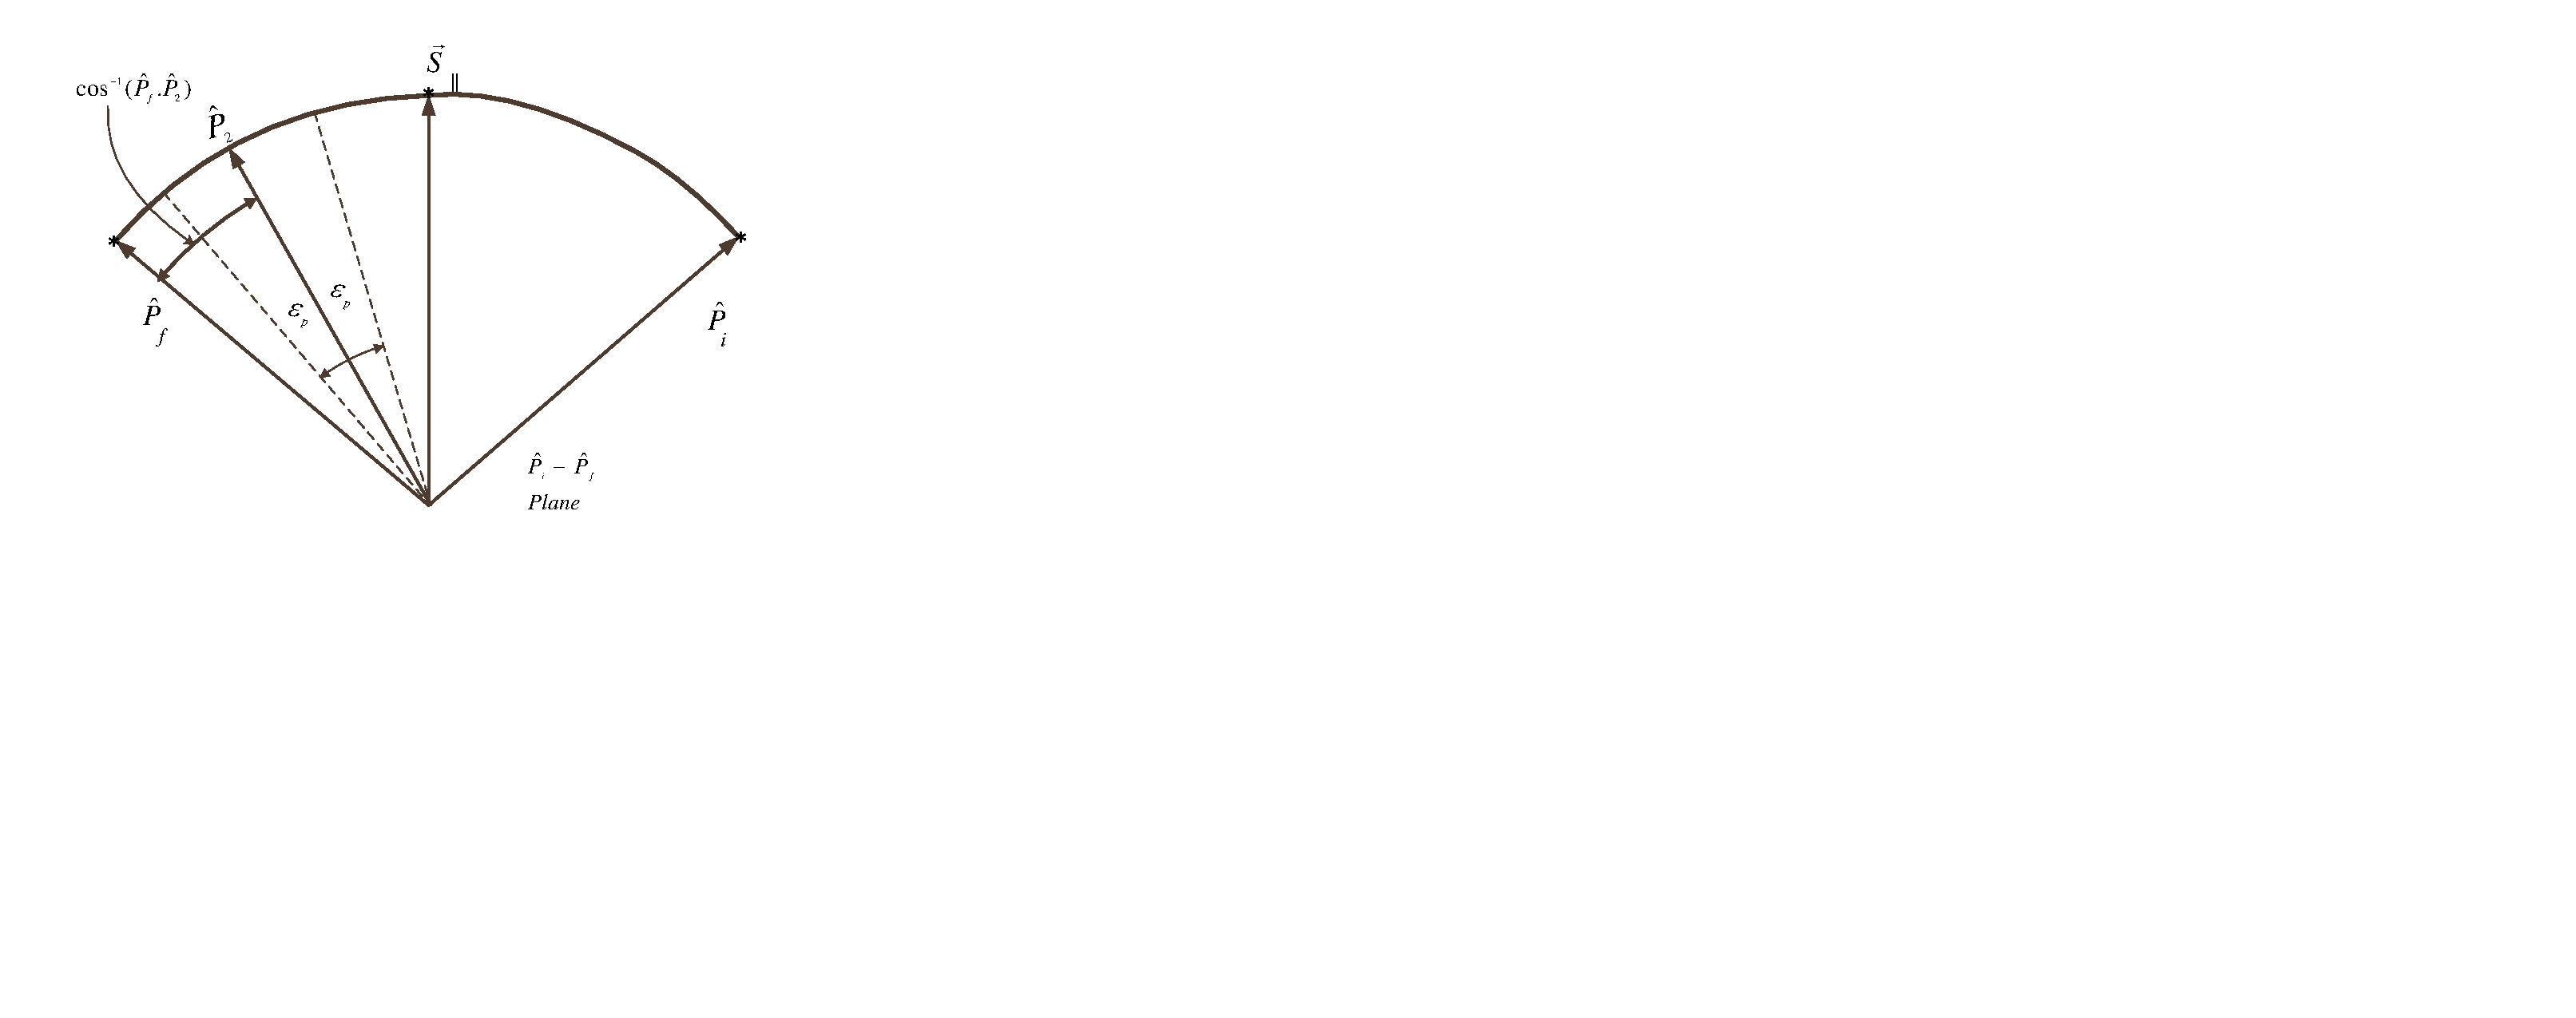
\includegraphics[width=2.3in]{./Figures/SVAS_4r}
			\end{center}
		\end{figure}
		%		\end{enumerate}
		%		\begin{enumerate}[4]
		\item The final slew is about the instrument boresight axis to go to the final attitude. 
	\end{enumerate}
	%	\end{enumerate}
	
	%-------------------------------------------------------------------------------------------------------------------------------------------------------------------
	
	\subsection{Summary of Algorithm} 
	
	\begin{enumerate}
		\item Slew around the eigenaxis,$\hat{e}$, through angle:
		
		\begin{equation}\label{phi1}
		\phi_1=\left\{
		\begin{array}{ll}
		\cos^{-1}(\hat{P}._G\hat{S}_{||})-\epsilon_p& when\  \cos^{-1}(\hat{P}._G\hat{S}_{||})-\epsilon_p\leq \pi\\
		\cos^{-1}(\hat{P}._G\hat{S}_{||})-\epsilon_p-2\pi& when\ \cos^{-1}(\hat{P}._G\hat{S}_{||})-\epsilon_p>\pi\\
		\end{array}
		\right.
		\end{equation}
		\item Slew around the $\hat{S}$ via:
		\begin{equation}\label{phi2}
		\phi_2=\left\{
		\begin{array}{ll}
		2\tan^{-1}(\frac{\epsilon_p}{\sin\alpha})& when\  \alpha\neq 0\\
		\pi& when\ \alpha=0\\
		\end{array}
		\right.
		\end{equation}
		\item Slew about the $\hat{e}$ through angle:
		\begin{equation}\label{phi3}
		\phi_3=\left\{
		\begin{array}{ll}
		\cos^{-1}(_G\hat{P}_f.\hat{P}_2)& when\  _G\hat{P}_f.\hat{P}_2\geq 0\\
		\cos^{-1}(_G\hat{P}_f.\hat{P}_2)-2\pi& when\ _G\hat{P}_f.\hat{P}_2<0\\
		\end{array}
		\right.
		\end{equation}
		
		\item Perform the final rotation, $\phi_4$, about the instrument boresight axis to adjust the attitude. 
	\end{enumerate}
	
	%-------------------------------------------------------------------------------------------------------------------------------------------------------------------
	
	\begin{figure}[H]
		\begin{center}
			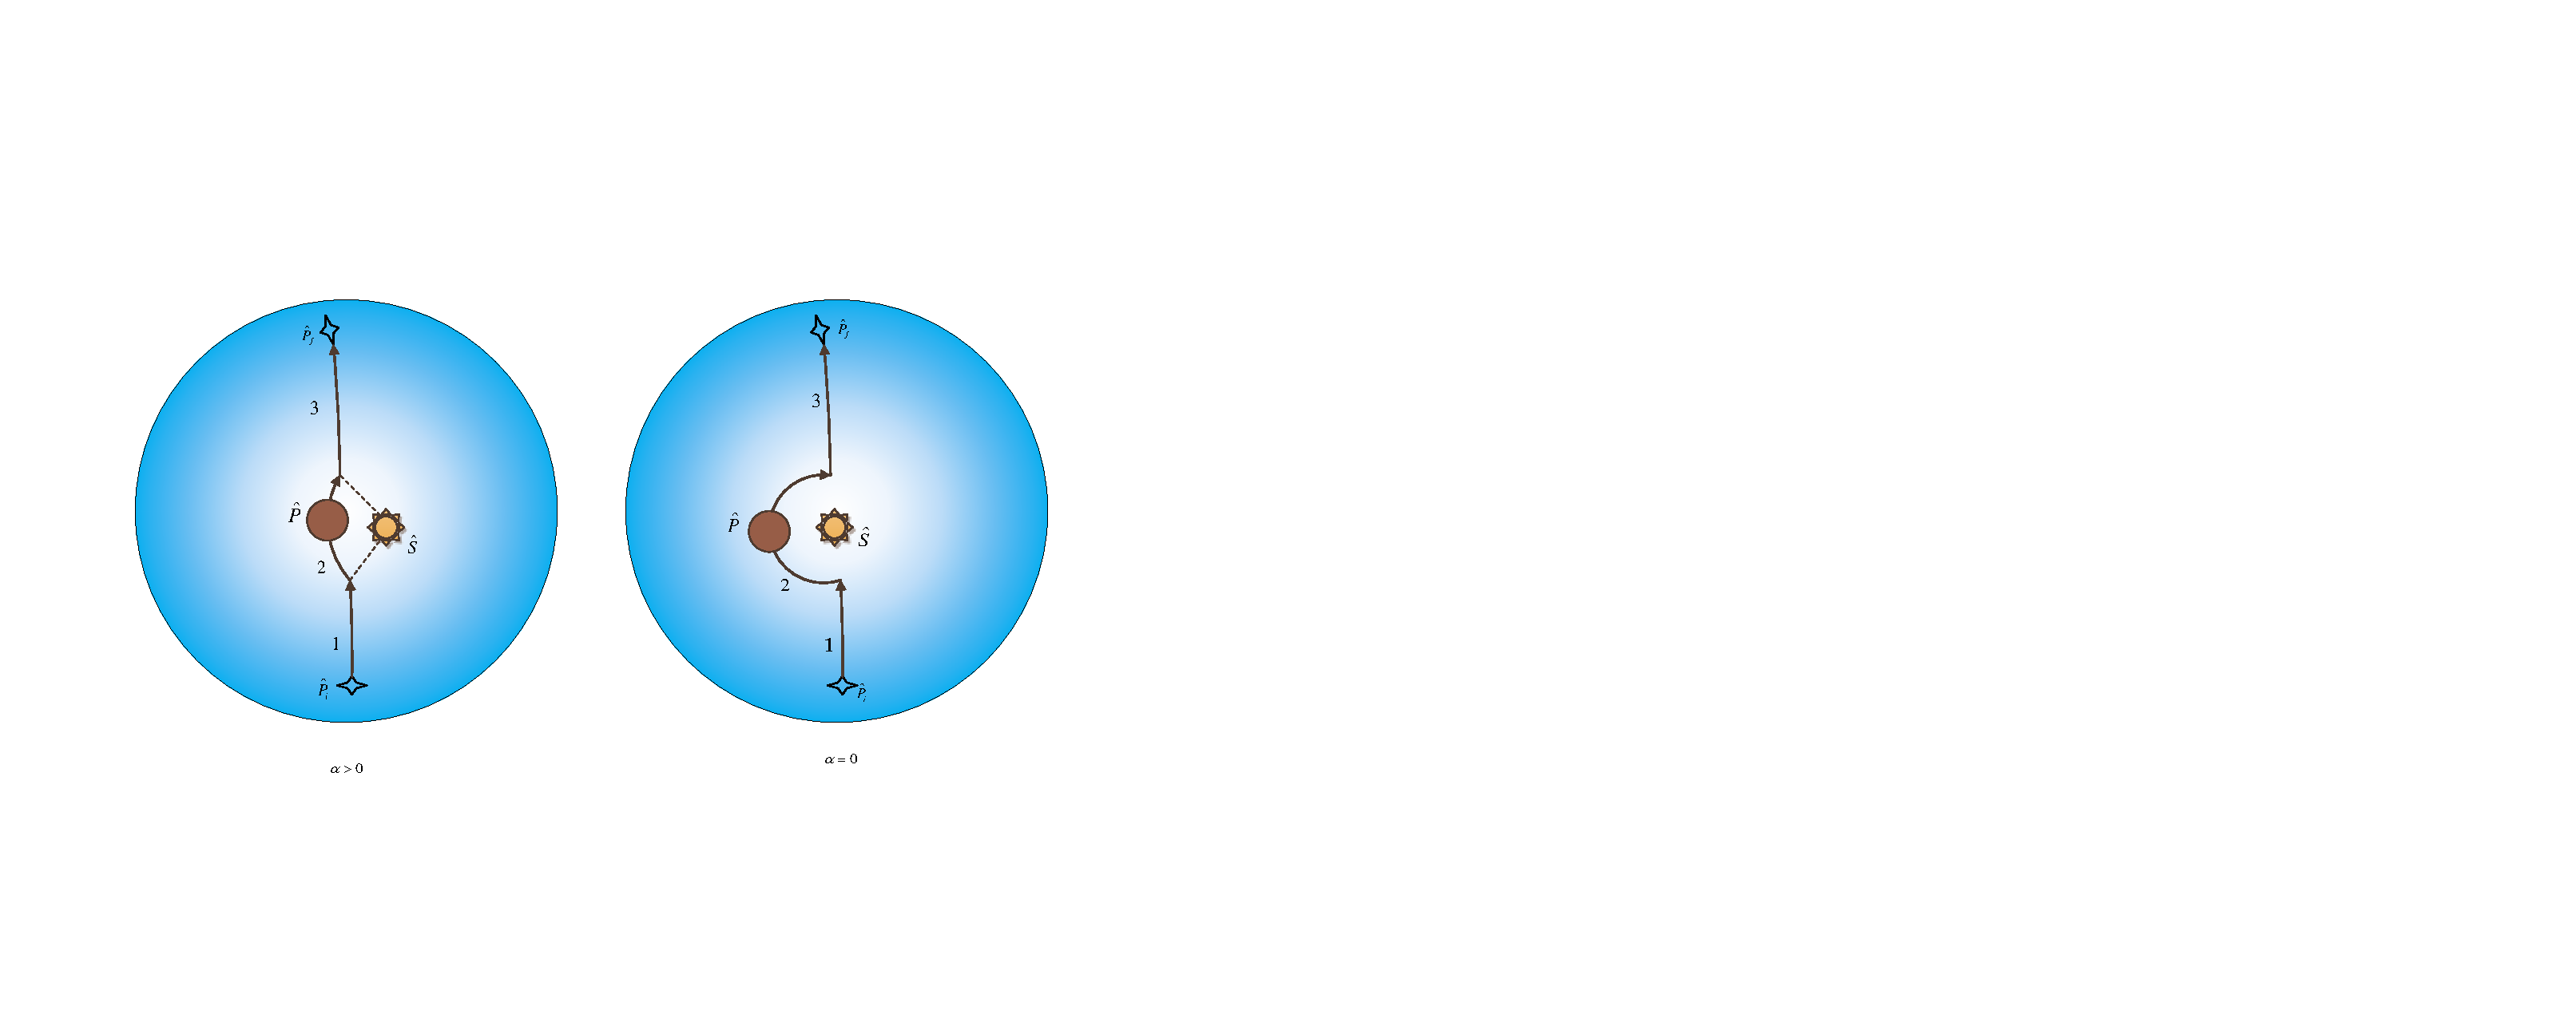
\includegraphics[width=6in]{./Figures/SASSchematic3}
		\end{center}
	\end{figure}
	
	%-------------------------------------------------------------------------------------------------------------------------------------------------------------------
	
	\section{Steering Laws} 
	
	\subsection{Case 1: Single-Axis, Agile Slew Maneuver with Velocity and Acceleration Constraints.}	 
	
	%-------------------------------------------------------------------------------------------------------------------------------------------------------------------
	
	\subsubsection{Problem Statement}
	
	Consider the motion of a \textcolor{blue}{rigid} spacecraft around a given inertially-fixed axis, $_G\hat{e}=[e_x,e_y,e_z]^T$. The problem of minimum-time slew maneuver around the $\hat{e}$ axis can be formulated as
	
	\begin{equation}\label{costfunction}
	\underset{u}{Minimze}\ J[x(.), u(.), t_f]=\int_{t0}^{t_f} dt,
	\end{equation}
	
	subject to the following dynamic constraint
	
	\begin{equation}\label{system}
	\Sigma:\left\{
	\begin{array}{l}
	\dot{x}_1=x_2, \\
	\dot{x}_2=M/I_{\hat{e}}^{G/G*}=u, \\
	\end{array}
	\right.
	\end{equation}
	
	where $x_1 \triangleq\phi$ and $x_2=\dot{\phi}$. 
	
	\begin{figure}[H]
		\begin{center}
			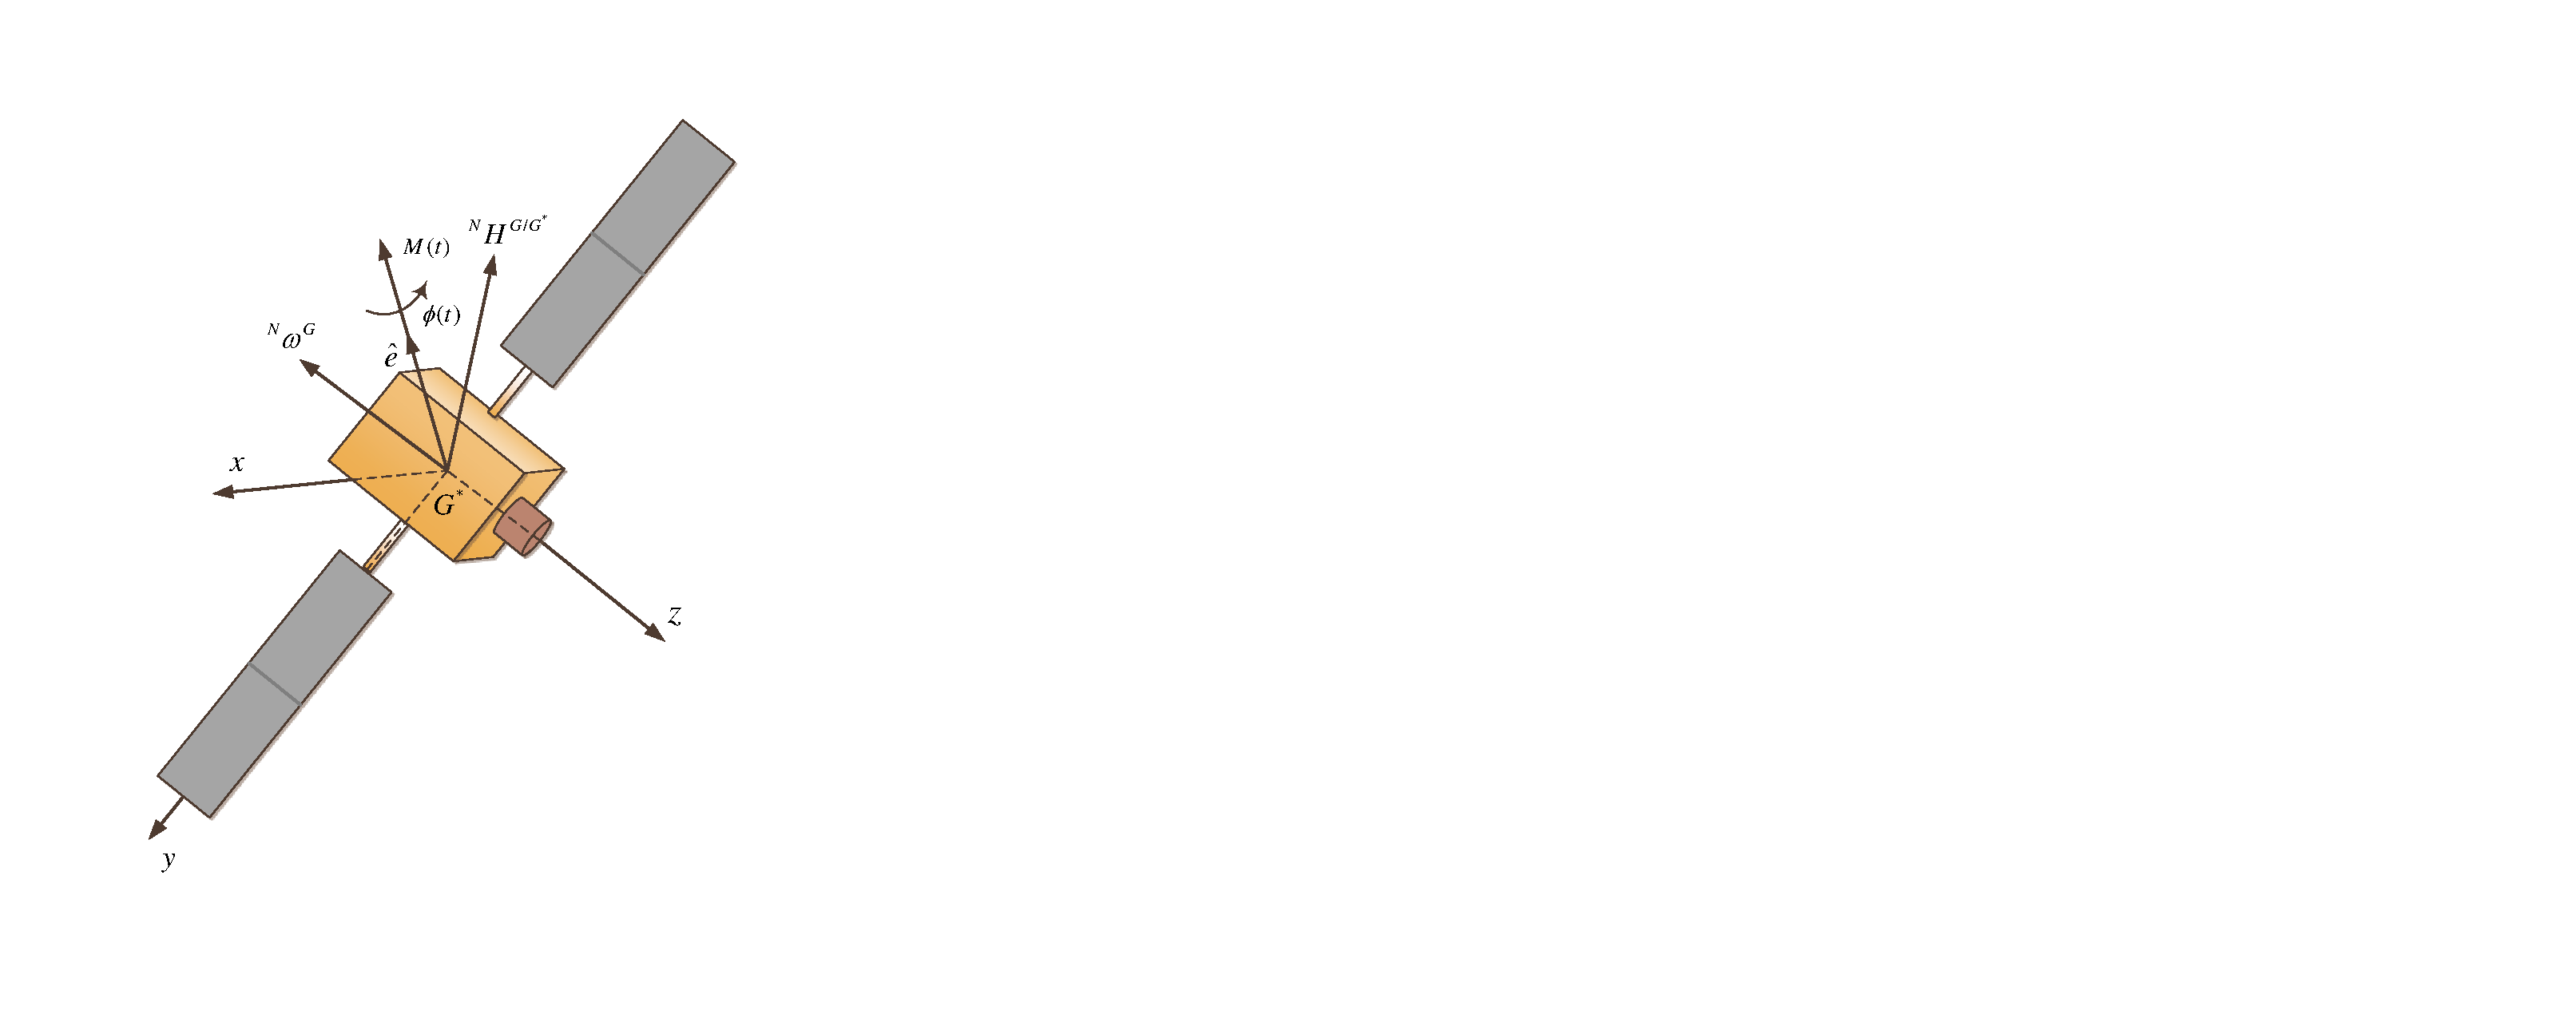
\includegraphics[width=2.25in]{./Figures/Spacecraft}  
		\end{center}    
	\end{figure}
	
	%-------------------------------------------------------------------------------------------------------------------------------------------------------------------
	
	\subsubsection{Velocity and Acceleration Constraints}
	
	The boundary conditions are
	\begin{equation}\label{Bcs}
	BCs:\left\{
	\begin{array}{l}
	\phi(t_0)=0, \phi(t_f)=\phi_{f},\\
	\dot{\phi}(t_0)=\dot{\phi}_{0},\dot{ \phi}(t_f)=\dot{\phi}_{f}, \\
	\end{array}
	\right.
	\end{equation}
	and velocity (state) and acceleration (control) constraints are
	\begin{equation}\label{constraints1}
	C_1:\left\{
	\begin{array}{l}
	|x_2=\dot{\phi}|\leq \dot{\phi}_{max},\\
	|u=\ddot{\phi}|\leq \ddot{\phi}_{max},\\
	\end{array}
	\right.
	\end{equation}
	in which
	\begin{equation}
	\dot{\phi}_{max}=[I^{w/w^*}]^{-1}[^NH^{G/G*}-(I^{G/G*}+I^{w/w*})^N\omega^G]/(e_x+e_y+e_z),
	\end{equation}
	
	%-------------------------------------------------------------------------------------------------------------------------------------------------------------------
	
	and
	\begin{equation}\label{phiddotmax}
	\ddot{\phi}_{max}=_B\hat{e}^T\  _BM_{max}/I_{\hat{e}}^{G/G*},
	\end{equation}
	where $^NH^{G/G*}$ is the total angular momentum of the gyrostat with respect to its center of mass, $G^*$, in the $N$-frame. $I^{G/G^*}$ and $I^{w/w*}$ represent the inertia dyadic of the gyrostat and reaction wheel with respect to their center of masses, respectively. $_BM_{max}$ is the maximum generated torque along the body-axes in the body frame. \\
	%Find the optimal steering laws: $^Bq^R$, $^B\omega^R$, and $^B\alpha^R$.
	%			\vspace{0.5in}
	
	{\bf Find:} $\phi(t)$, $\dot{\phi}(t)$, and $\ddot{\phi}(t)$.
	
	%-------------------------------------------------------------------------------------------------------------------------------------------------------------------
	
	Using the Pontryagin's minimum principle (PMP), we derive the necessary conditions for the optimal solution as follows:
	\begin{enumerate}
		\item State Eqs.:
		\begin{equation}
		\left\{
		\begin{array}{l}
		\dot{x}_1=x_2, \\
		\dot{x}_2=u, \\
		\dot{x}_3=(x_2+\dot{\phi}_{max})^2\mathbb{U}(-x_2-\dot{\phi}_{max})+(\dot{\phi}_{max}-x_2)^2\mathbb{U}(x_2-\dot{\phi}_{max}),
		\end{array}
		\right.
		\end{equation}
		where the unit step function, $\mathbb{U}$, is defined as
		\begin{equation}
		\mathbb{U}(X)=\left\{
		\begin{array}{l}
		1,   X>0, \\
		0,   X\leq 0.
		\end{array}
		\right.
		\end{equation}
		Note:  ($x_3(t_0)=x_3(t_f)=0$ \& $x_3(t)\geq 0$ ) $\rightarrow x_3(t)=0, t\in[t_0, t_f]$. 
		%				Note:  ($x_3(t_0)=x_3(t_f)=0$ \& $x_3(t)\geq 0$ ) $\rightarrow x_3(t)=0, \foral t\in[t_0, t_f]. $  
		
		\item Hamiltonian:
		
		\begin{equation}
		\begin{split}
		\mathscr{H}=& 1+\lambda_1x_2+\lambda_2u+\lambda_3\Big[(x_2+\dot{\phi}_{max})^2\mathbb{U}(-x_2-\dot{\phi}_{max})\\
		& (\dot{\phi}_{max}-x_2)^2\mathbb{U}(x_2-\dot{\phi}_{max})\Big]
		\end{split}
		\end{equation}
		%			\end{enumerate}
		
		%-------------------------------------------------------------------------------------------------------------------------------------------------------------------
		
		%			\begin{enumerate}
		%				\conti
		%				\small{
		\item Costate Eqs.:
		\begin{equation}
		\left\{\begin{array}{l}
		\dot{\lambda}_1=-\frac{\partial{\mathscr{H}}}{\partial{x_1}}=0,\\
		\dot{\lambda}_2=-\frac{\partial{\mathscr{H}}}{\partial{x_2}}=-\lambda_1-2\lambda_3(x_2+\dot{\phi}_{max})\mathbb{U}(-x_2-\dot{\phi}_{max})\\
		+2\lambda_3(\dot{\phi}_{max}-x_2)\mathbb{U}(x_2-\dot{\phi}_{max}),\\
		\dot{\lambda}_3=-\frac{\partial{\mathscr{H}}}{\partial{x_3}}=0.\\
		\end{array}
		\right.
		\end{equation}
		\item Applying the Pontryagin's minimum principle (PMP),
		\begin{equation}
		u^*=arg \underset{u\in\mathcal{U}}{min} \mathscr{H},
		\end{equation}
		where $\mathcal{U}$ defines the domain of feasible controls. The optimal control can be determined as
		\begin{equation}
		u^*(t)=\left\{
		\begin{array}{lI}
		\ddot{\phi}_{max}&\lambda_2<0,\\
		?& \lambda_2=0,\\
		-\ddot{\phi}_{max}&\lambda_2>0.
		\end{array}
		\right.
		\end{equation}
		%				}
		%			\end{enumerate}
		%			\seti
		This is a {\it singular arc} optimal control problem.
		
		%-------------------------------------------------------------------------------------------------------------------------------------------------------------------
		
		\item Determining the optimal control in the singular arc:
		\begin{equation}
		\frac{d^2}{dt^2}\Big(\frac{\partial \mathscr{H}}{\partial u}\Big)=\ddot{\lambda}_2=0\rightarrow \dot{x}_2=0\rightarrow u^*=0
		\end{equation}
		\item Checking the Generalized Legendre-Clebsch condition for optimality:
		\begin{equation}
		(-1)^2\frac{\partial}{\partial u}\Big[\frac{d^2}{dt^2}\Big(\frac{\partial \mathscr{H}}{\partial u}\Big)\Big]=1\geq 0
		\end{equation}
		\item The transversality condition:
		\begin{equation}
		\mathscr{H}|_{(*,t_f)}=0\  \text{and} \ \mathscr{H}\neq\mathscr{H}(t)\rightarrow \mathscr{H}=0, \forall t\in[t_0, t_f].
		\end{equation}
	\end{enumerate}
	%	\seti
	
	%-------------------------------------------------------------------------------------------------------------------------------------------------------------------
	
	\subsubsection{Steering Profiles}
	
	\begin{itemize}
		\item Angular acceleration profile (bang-off-bang):
	\end{itemize}
	\begin{equation}\label{phidd_cons}
	\ddot{\phi}(t)=u=\left\{
	\begin{array}{ll}
	\ddot{\phi}_{max}& when\  t_0\leq t\leq t_1,\\
	0& when\  t_1\leq t \leq t_2,\\
	-\ddot{\phi}_{max}& when \ t_2\leq t\leq t_f.
	\end{array}
	\right.
	%			\begin{minipage}{0.35\textwidth}
	%			\end{minipage}
	\end{equation}
	%			\begin{figure}[H]
	%				\begin{center}
	%					\includegraphics[width=1.5in]{./Figures/bang_off_bang
	%				\end{center}
	%			\end{figure}
	\begin{itemize}
		\item Angular velocity profile:
	\end{itemize}
	\begin{equation}\label{phid_cons}
	\dot{\phi}(t)=\left\{
	\begin{array}{ll}
	\dot{\phi}_0+\ddot{\phi}_{max}(t-t_0)& when\  t_0\leq t\leq t_1,\\
	\dot{\phi}_{max}& when\  t_1\leq t \leq t_2,\\
	\dot{\phi}_{max}-\ddot{\phi}_{max}(t-t_2)& when \ t_2\leq t\leq t_f.
	\end{array}
	\right.
	\end{equation}
	\begin{itemize}
		\item Angular position profile:
	\end{itemize}
	\begin{equation}\label{phi_cons}
	\phi(t)=\left\{
	\begin{array}{ll}
	\dot{\phi}_0(t-t_0)+\frac{1}{2}\ddot{\phi}_{max}(t-t_0)^2& when\  t_0\leq t\leq t_1,\\
	\phi(t_1)+ \dot{\phi}_{max}(t-t_1)& when\  t_1\leq t \leq t_2,\\
	\phi(t_2)+\dot{\phi}_{max}(t-t_2)-\frac{1}{2}\ddot{\phi}_{max}(t-t_2)^2& when \ t_2\leq t\leq t_f.
	\end{array}
	\right.
	\end{equation}
	
	%-------------------------------------------------------------------------------------------------------------------------------------------------------------------
	
	\begin{itemize}
		\item Using the conditions, $\dot{\phi}(t_1)=\dot{\phi}_{max}$, $\dot{\phi}(t_f)=\dot{\phi}_f$, $\phi(t_f)=\phi_f$, we can determine switching times $t_1$, $t_2$, and final time $t_f$ as:
	\end{itemize}
	\begin{equation}\label{t1cons}
	t_1=t_0+\frac{\dot{\phi}_{max}-\dot{\phi}_0}{\ddot{\phi}_{max}},
	\end{equation}
	\begin{equation}\label{t2cons}
	\begin{split}
	t_2=&t_1+\frac{1}{\dot{\phi}_{max}}\Big[ \phi_f-\dot{\phi}_0(t_1-t_0)-\frac{1}{2}\ddot{\phi}_{max}(t_1-t_0)^2\\
	&-\frac{\dot{\phi}_{max}(\dot{\phi}_{max}-\dot{\phi}_f)}{\ddot{\phi}_{max}}+\frac{(\dot{\phi}_{max}-\dot{\phi}_f)^2}{2\ddot{\phi}_{max}} \Big],
	\end{split}
	\end{equation}
	and
	\begin{equation}\label{tfcons}
	t_f=t_1+\frac{1}{\dot{\phi}_{max}}\Big[ \phi_f-\dot{\phi}_0(t_1-t_0)-\frac{1}{2}\ddot{\phi}_{max}(t_1-t_0)^2+\frac{(\dot{\phi}_{max}-\dot{\phi}_f)^2}{2\ddot{\phi}_{max}} \Big].
	\end{equation}
	
	%-------------------------------------------------------------------------------------------------------------------------------------------------------------------
	
	\begin{itemize}
		\item Steering profiles:
		\begin{equation}
		^Nq^D(t)=[e_x\sin\frac{\phi(t)}{2}, e_y\sin\frac{\phi(t)}{2}, e_z\sin\frac{\phi(t)}{2}, \cos\frac{\phi(t)}{2}]^T
		\end{equation}
		\begin{equation}
		^N_G\omega^D(t)=\dot{\phi}(t)_G\hat{e}
		\end{equation}
		\begin{equation}
		^N_G\alpha^D(t)=\ddot{\phi}(t)_G\hat{e}
		\end{equation}
	\end{itemize}
	
	%-------------------------------------------------------------------------------------------------------------------------------------------------------------------
	
	\subsection{Case 2: Single-Axis, Agile Slew Maneuver with Acceleration Constraint} 
	
	\subsubsection{Problem Statement} 
	
	Consider the optimal control problem described by Eqs.(\ref{costfunction}), (\ref{system}), (\ref{Bcs}), and subject to control constraint
	\begin{equation}
	C_2: \ |u=\ddot{\phi}|\leq \ddot{\phi}_{max}.
	\end{equation}
	
	{\bf Find:} $\phi(t)$, $\dot{\phi}(t)$, and $\ddot{\phi}(t)$.
	
	%-------------------------------------------------------------------------------------------------------------------------------------------------------------------
	
	\begin{itemize}
		\item Angular acceleration about the $\hat{e}$ axis:
	\end{itemize}
	\begin{equation}\label{alpha}
	\ddot{\phi}(t)=\ddot{\phi}_{max}\mathbb{U}(t_0)- 2\ddot{\phi}_{max}\mathbb{U}(t-t_1)
	\end{equation}
	
	\begin{center}
		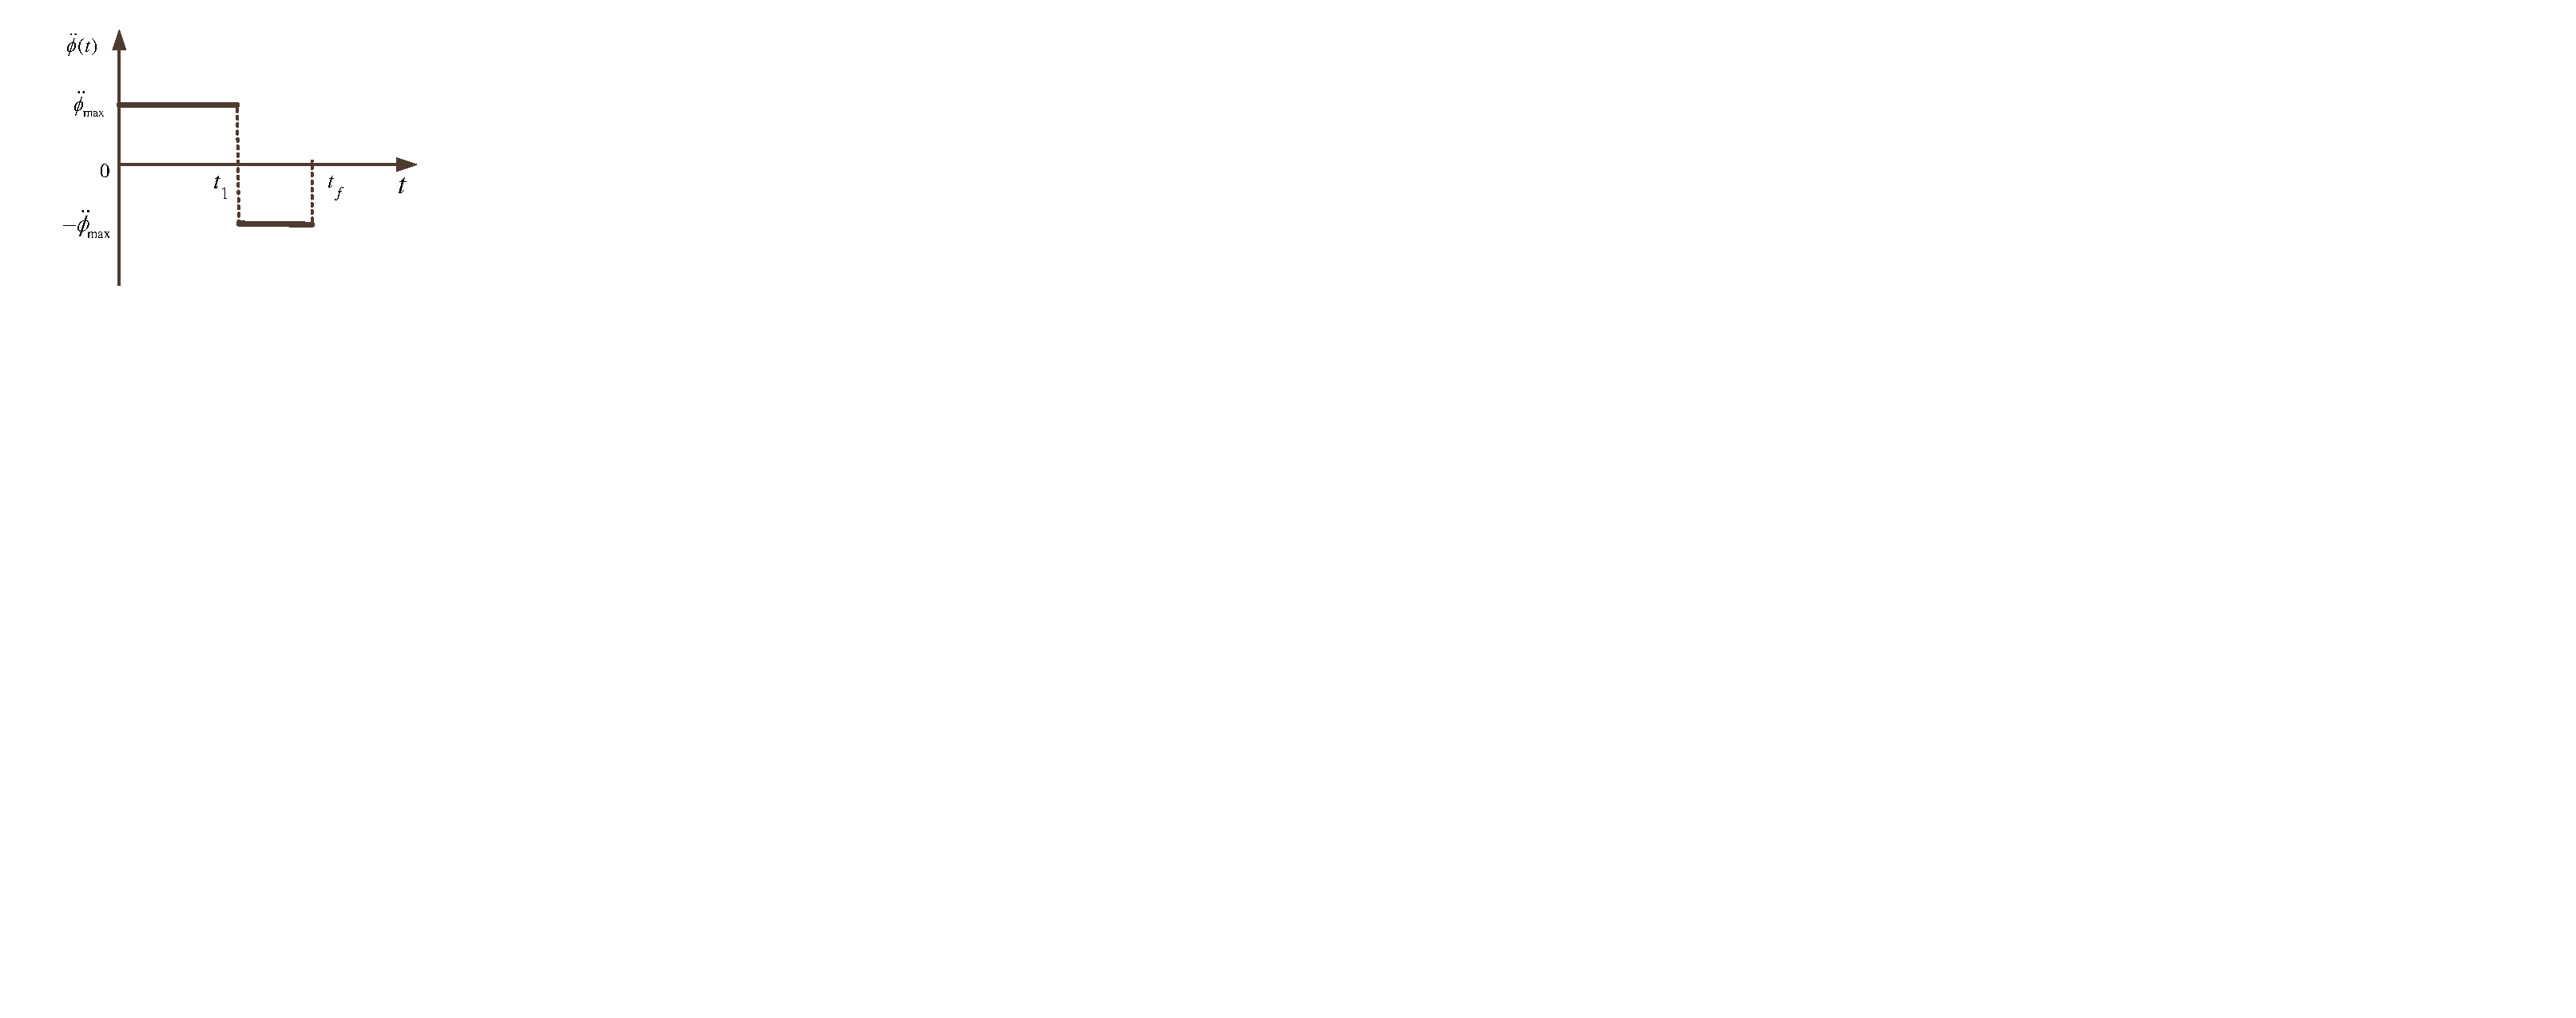
\includegraphics[width=2in]{./Figures/Bang_bang}      
	\end{center}
	
	where the switching and the final times are given by
	\begin{equation}
	t_1=t_0-\frac{\dot{\phi}_{0}}{\ddot{\phi}_{max}}+\frac{\sqrt{\ddot{\phi}_{max}^2(2\ddot{\phi}_{max}\phi_{f}+\dot{\phi}_{f}^2+\dot{\phi}_{0}^2)}}{\sqrt{2}\ddot{\phi}_{max}^2}
	\end{equation}
	
	%-------------------------------------------------------------------------------------------------------------------------------------------------------------------
	
	and
	\begin{equation}
	t_f=t_0-\frac{\dot{\phi}_{f}+\dot{\phi}_{0}}{\ddot{\phi}_{max}}+\frac{\sqrt{2}\sqrt{\ddot{\phi}_{max}^2(2\ddot{\phi}_{max}\phi_{f}+\dot{\phi}_{ef}^2+\dot{\phi}_{0}^2)}}{\ddot{\phi}_{max}^2}
	\end{equation}
	\begin{itemize}
		\item Angular velocity about the $\hat{e}$ axis:
	\end{itemize}
	\begin{equation}\label{omega}
	\dot{\phi}(t)=\dot{\phi}_{0}+\ddot{\phi}_{max}(t-t_0)\mathbb{U}(t_0)- 2\ddot{\phi}_{max}(t-t_1)\mathbb{U}(t-t_1)
	\end{equation}
	\begin{itemize}
		\item Angular position about the $\hat{e}$ axis:
	\end{itemize}
	\begin{equation}\label{phi}
	\begin{split}
	\phi(t)&=\dot{\phi}_{0}(t-t_0)+\ddot{\phi}_{max}\frac{(t-t_0)^2}{2}\mathbb{U}(t_0)\\
	&- 2\ddot{\phi}_{max}\frac{(t-t_1)^2}{2}\mathbb{U}(t-t_1)
	\end{split}
	\end{equation}
	
	%-------------------------------------------------------------------------------------------------------------------------------------------------------------------
	
	\subsubsection{The First Slew Maneuver: A single-axis nonrest-to-rest maneuver around the $\hat{e}$}
	
	\begin{itemize}
		\item The BCs: 
	\end{itemize}
	\begin{equation}\label{Bc1}
	\dot{\phi}(t_0)=\dot{\phi}_{0},\phi(t_0)=0, \dot{\phi}(t_{f1})=0,\phi(t_{f1})=\phi_1.
	\end{equation}
	
	The switching time, $t_{11}$, and minimum-time, $t_{f1}$, are
	\begin{equation}\label{t11}
	t_{11}=t_0-\frac{\dot{\phi}_0}{\ddot{\phi}_{max}}+\frac{\sqrt{\ddot{\phi}_{max}^2(2\ddot{\phi}_{max}\phi_1+\dot{\phi}_{0}^2)}}{\sqrt{2}\ddot{\phi}_{max}^2}
	\end{equation}
	\begin{equation}\label{tf1}
	t_{f1}=t_0-\frac{\dot{\phi}_0}{\ddot{\phi}_{max}}+\frac{\sqrt{2\ddot{\phi}_{max}^2(2\ddot{\phi}_{max}\phi_1+\dot{\phi}_{0}^2)}}{\ddot{\phi}_{max}^2}
	\end{equation}
	The $\ddot{\phi}(t)$, $\dot{\phi}(t)$, and  $\phi(t)$,  can be found by substituting the boundary conditions given by (\ref{Bc1}) and $t_{11}$ and $t_{f1}$ in to Eqs. (\ref{alpha}), (\ref{omega}), and (\ref{phi}), respectively.
	
	%-------------------------------------------------------------------------------------------------------------------------------------------------------------------
	
	\subsubsection{The Second Slew Maneuver: A rest-to-rest maneuver around the sun vector} 
	
	\begin{itemize}
		\item The BCs: 
	\end{itemize}
	\begin{equation}\label{Bc2}
	\dot{\phi}(t_0)=0,\phi(t_0)=0, \dot{\phi}(t_{f2})=0,\phi(t_{f2})=\phi_2.
	\end{equation}
	The switching time, $t_{12}$, and the minimum-time, $t_{f2}$, are
	\begin{equation}\label{t21}
	t_{12}=t_0-\frac{\sqrt{\phi_2}}{\ddot{\phi}_{max}}
	\end{equation}
	\begin{equation}\label{tf2}
	t_{f2}=t_0-\frac{2\sqrt{\phi_2}}{\ddot{\phi}_{max}}
	\end{equation}
	The $\ddot{\phi}(t)$, $\dot{\phi}(t)$, and  $\phi(t)$,  can be found by substituting the boundary conditions given by (\ref{Bc2}) and $t_{12}$ and $t_{f2}$ in to Eqs. (\ref{alpha}), (\ref{omega}), and (\ref{phi}), respectively.
	
	%-------------------------------------------------------------------------------------------------------------------------------------------------------------------
	
	\subsubsection{The Third Slew Maneuver: A single-axis rest-to-nonrest maneuver around the $\hat{e}$}
	
	
	\begin{itemize}
		\item The BCs: 
	\end{itemize}
	\begin{equation}\label{Bc3}
	\dot{\phi}(t_0)=0,\phi(t_0)=0, \dot{\phi}(t_{f3})=\dot{\phi}_{f},\phi(t_{f3})=\phi_3.
	\end{equation}
	The switching time, $t_{13}$, and the minimum-time, $t_{f3}$, are
	\begin{equation}\label{t31}
	t_{13}=t_0+\frac{\sqrt{\ddot{\phi}_{max}^2(2\ddot{\phi}_{max}\phi_3+\dot{\phi}_{f}^2)}}{\sqrt{2}\ddot{\phi}_{max}^2}
	\end{equation}
	\begin{equation}\label{tf3}
	t_{f3}=t_0-\frac{\dot{\phi}_{f}}{\ddot{\phi}_{max}}+\frac{\sqrt{2\ddot{\phi}_{max}^2(2\ddot{\phi}_{max}\phi_3+\dot{\phi}_{f}^2)}}{\ddot{\phi}_{max}^2}
	\end{equation}
	The $\ddot{\phi}(t)$, $\dot{\phi}(t)$, and  $\phi(t)$,  can be found by substituting the boundary conditions given by (\ref{Bc3}) and $t_{13}$ and $t_{f3}$ in to Eqs. (\ref{alpha}), (\ref{omega}), and (\ref{phi}), respectively.
	
	%-------------------------------------------------------------------------------------------------------------------------------------------------------------------
	
	\section{Numerical simulation} 
	
	\section{Conclusion}
	
	\section{Acknowledgment}
	
	\appendix
	\section*{Appendix: Title here}
	
	\subsection*{Miscellaneous Physical Dimensions}
	
	\bibliographystyle{AAS_publication}   % Number the references.
	\bibliography{references_SAA}   % Use references.bib to resolve the labels.
	
	
	
\end{document}
